\documentclass[tikz,border=5pt]{standalone}
\usepackage{tikz}
\usetikzlibrary{arrows.meta}
\definecolor{nebula}{HTML}{6366F1}
\definecolor{spark}{HTML}{14B8A6}
\definecolor{ink}{HTML}{334155}
\begin{document}
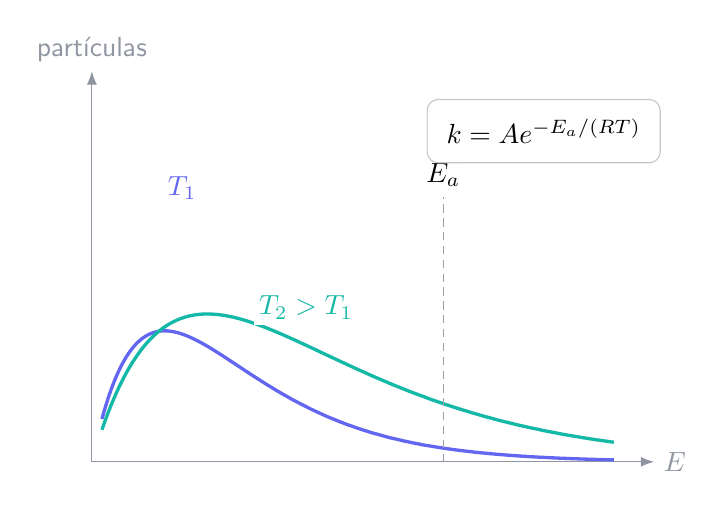
\begin{tikzpicture}[font=\sffamily,>=Latex,x=.85cm,y=.8cm]
  \draw[->,ink!55] (0,0)--(8.4,0) node[right] {$E$};
  \draw[->,ink!55] (0,0)--(0,6.2) node[above] {partículas};
  \draw[very thick,nebula,domain=.15:7.8,samples=150,smooth] plot(\x,{5.2*\x*exp(-.92*\x)});
  \draw[very thick,spark,domain=.15:7.8,samples=150,smooth] plot(\x,{3.7*\x*exp(-.58*\x)});
  \draw[densely dashed,ink!50] (5.25,0)--(5.25,4.2);
  \node[fill=white,inner sep=2pt] at (5.25,4.55) {$E_a$};
  \node[text=nebula,fill=white,inner sep=2pt] at (1.35,4.35) {$T_1$};
  \node[text=spark,fill=white,inner sep=2pt] at (3.2,2.45) {$T_2>T_1$};
  \node[draw=ink!30,rounded corners=4pt,fill=white,inner sep=7pt] at (6.75,5.25)
    {$k=Ae^{-E_a/(RT)}$};
\end{tikzpicture}
\end{document}
